\documentclass[usenames,dvipsnames,fleqn,leqno,10pt, pdflatex]{beamer}
%\usetheme[professionalfonts]{Boadilla}
\usetheme{metropolis}
\setsansfont[BoldFont={Source Sans Pro Semibold}, Numbers={OldStyle}]{Source Sans Pro}
%\usepackage{fontspec}


\metroset{block=fill,background=light}
\setbeamertemplate{blocks}[rounded]

\usepackage{cite}
\usepackage{pgfplots}
%\usepackage[symbol]{footmisc}
%\setmainfont{Liberation Serif}
%\setbeamertemplate{bibliography item}[text]
%\usepackage{graphicx}
\usepackage{bbding}
\setbeamertemplate{caption}[numbered]
\setbeamertemplate{footline}[text line]{%
\parbox{\linewidth}{\vspace*{-8pt}\hfill\insertshortauthor\hfill\insertpagenumber}}
\setbeamertemplate{navigation symbols}{}
%\author[bw]{}
\usepackage{amsmath}
\usepackage{amsthm}
\usepackage{upgreek}
\usepackage{isomath}
\usepackage[normalem]{ulem}
%\usepackage{comment}
\usepackage[USenglish]{babel}
\usepackage[activate={true,nocompatibility},final,tracking=true,factor=1100,stretch=10,shrink=10]{microtype}
\usepackage[]{xcolor}
\newcommand{\reals}{\mathbf{R}}
\newcommand{\complex}{\mathbf{C}}
\newcommand{\integers}{\mathbf{Z}}
\newcommand{\imag}{\mathrm{i}}
\DeclareMathOperator{\range}{range}
\DeclareMathOperator{\domain}{domain}
\DeclareMathOperator{\codomain}{codomain}
\DeclareMathOperator{\sspan}{span}
\usepackage{graphicx}

\definecolor{UNK-blue}{HTML}{004d86} 
\definecolor{UNK-gold}{HTML}{E4A115} 

\newenvironment{PenList}{
  \begin{enumerate}[\textcolor{UNK-blue}{\PencilRightDown}]
    \addtolength{\itemsep}{-0.0\itemsep}}
  {\end{enumerate}}
  
\setbeamertemplate{theorems}[unnumbered]
\newtheorem{myprop}{Proposition}
\newtheorem{idea}{Idea}
\newtheorem{describ}{Description}
\newtheorem{Homework}{Homework}
\newtheorem{myproof}{Proof}
\newtheorem{fakeproof}{Fake Proof}
%------------------
\title[] % (optional, only for long titles)
{\textcolor{black}{\textbf{A Let/choose example}} \\ 
\vspace{0.2in}
%\textcolor{black}{Mini-symposium} \\
%\textcolor{UNK-blue}{\textbf{University of Nebraska at Kearney}}
}

%\usepackage{amsmath}

\date{\today}


\makeatletter
\newcommand{\leqnomode}{\tagsleft@true\let\veqno\@@leqno}
\newcommand{\reqnomode}{\tagsleft@false\let\veqno\@@eqno}
\makeatother
\author[] % (optional, for multiple authors)
{Barton~Willis}
%\institute[UNK] % (optional)
%{
 % \inst{1}%
 %   Barton Willis \\
 %   Department of Mathematics and Statistics\\
 %   University Nebraska at Kearney  \\
 %   Kearney, Nebraska 68849  USA \\
 %   \phantom{xxxx}\\
  %  \href{mailto:willisb@unk.edu}{willisb@unk.edu}}
 



%\usepackage{hyperref}
\pgfplotsset{compat=1.18}
\begin{document}

\frame{\titlepage}

\begin{frame}{Can we make sense of this?}

\begin{myprop}
We have
\begin{equation*}
    \left(\forall \,\, a \in \reals\right)\left(\exists \,\,  m \in \reals\right)\left (\forall \,\, x \in \reals \right)\left(x^2 \geq a^2 + m (x-a) \right).
\end{equation*}
\end{myprop}

\begin{itemize}
    \item Puzzled? Good.
    \item Let's try GNAT (= Geometric, Numerical, Algebraic, and Thinking)
    \item But how to do that?
 \end{itemize}

\vfill

\end{frame}

\begin{frame}{G is for geometric}

The main event of our proposition is the inequality  \(x^2 \geq a^2 + m (x-a) \).

\begin{itemize}
   \item For given values of $m$ and $a$, geometrically this says the parabola $y = x^2$ is above or touching the line \(y = a^2 + m (x-a)\).
   
   \item Let's try $a=1$ and $m=3$. A graph is
   
   \begin{center}
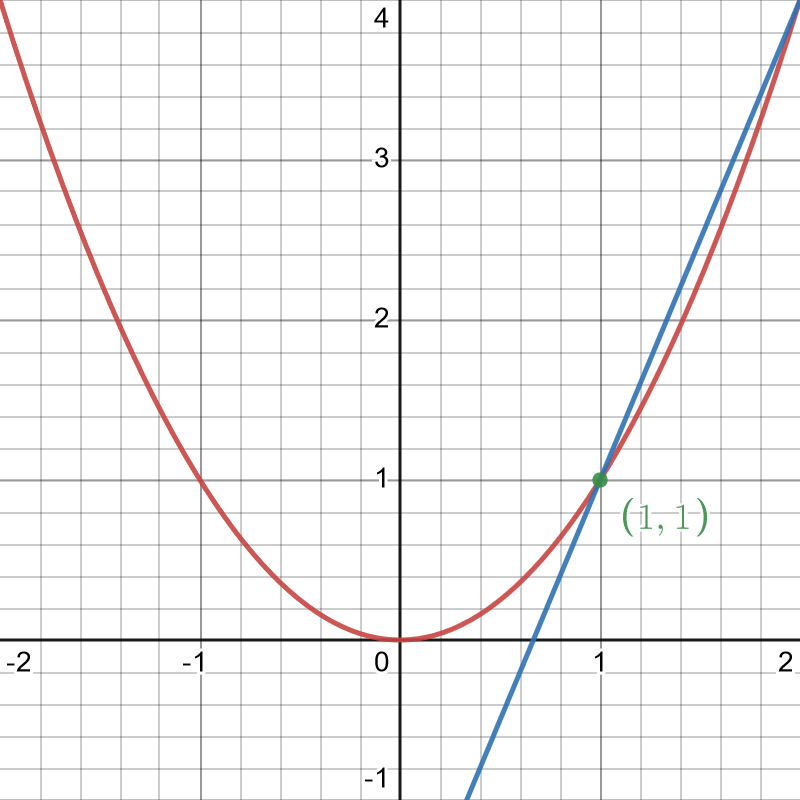
\includegraphics[scale=0.125]{desmos-graph(7).png}

\end{center}
\item To the left of one, the line is below the parabola, where is should be,

\item but just to the right of one, the line is \emph{above} the parabola, where it shouldn't be.

\item Apparently, the line is too steep.

\end{itemize}




\end{frame}

\begin{frame}{Let's be shallow}


\begin{itemize}
   \item Again, let's try $a=1$. Since $m=3$ was too big, let's try $m=1$. A graph is
   
   \begin{center}
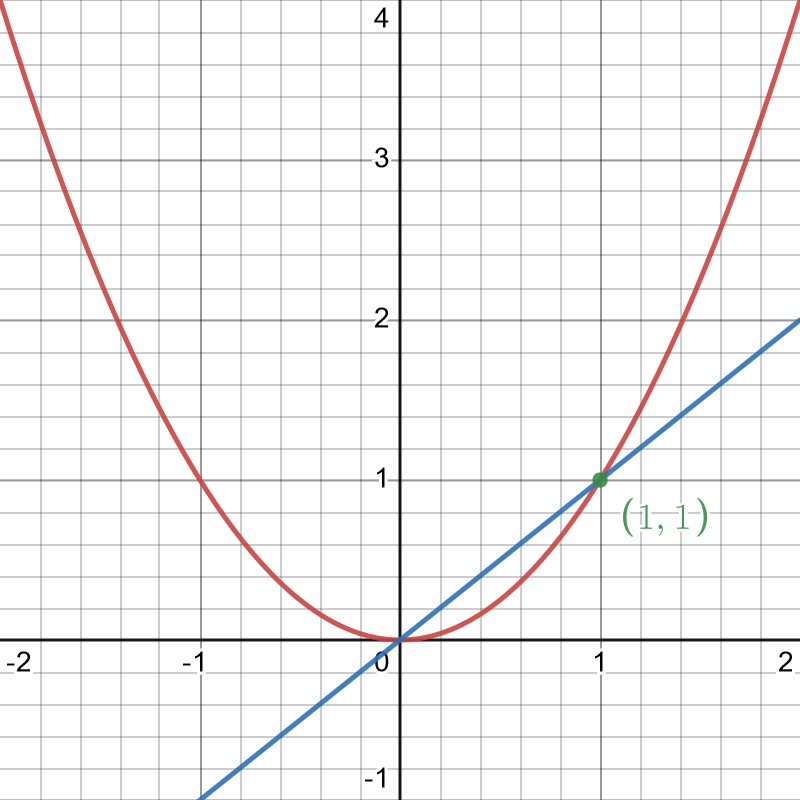
\includegraphics[scale=0.125]{desmos-graph(8).png}

\end{center}
\item To the left of one, the line is above the parabola, where it shouldn't  be,

\item but to the right of one, the line is \emph{below the parabola}, where it
should be.

\item OK: $m=1$ is too small and $m=3$ is too big. What do we choose?

\end{itemize}




\end{frame}

\begin{frame}{Let's not be shallow}

You guessed it: Choose $m=2$. The graph is 

  \begin{center}
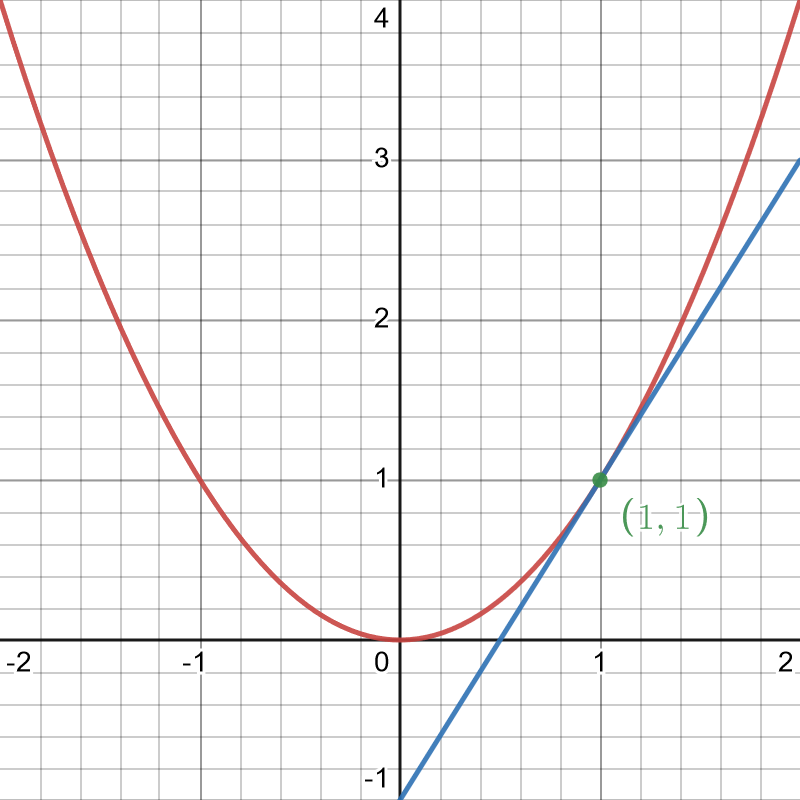
\includegraphics[scale=0.125]{desmos-graph(9).png}

\end{center}

Now the parabola is uniformly above or touching the line. Apparently, the magic choice for $m$ is two.

\begin{PenList}
\item Choices are hard. 

\item Like a Jeep, for $m$ there is only one (possible value).

\item Choose $m = 2 + \frac{1}{10^{100}}$, the inequality will not be satisfied for some
value of $x$ or $a$.

\end{PenList}
\end{frame}

\begin{frame}{G is also for Generalization}

\textbf{Question} OK, when $a=1$, we need to choose $m=2$. What's the story for other values of $a$?

\textbf{Answer} Sure.  We need to choose the line to be the \emph{tangent line}. Thus in the general case, we need to choose $m = 2 a$

\vfill

\end{frame}
\begin{frame}{A is for algebraic}

\begin{myprop}We have
$$
\left(\forall \,\, a \in \reals\right)\left(\exists \,\, m \in \reals\right)\left (\forall x \in \reals \right) \left(x^2 \geq a^2 + m (x-a) \right).
$$
\end{myprop}

\begin{myproof} Let $a \in \reals$. Choose $m = 2 a$. Let $x \in \reals$. We have
\begin{align*}
    \left[x^2 \geq a^2 + m (x -a) \right] &\equiv \left[x^2 \geq a^2 + 2a  (x -a) \right],
       &\mbox{(substitution)}\\
       &\equiv \left[x^2 \geq 2 a x - a^2\right], &\mbox{(expand)}\\
        &\equiv \left[x^2 - 2 a x + a^2  \geq 0 \right], &\mbox{(subtraction)}\\
        &\equiv \left[(x-a)^2  \geq 0 \right ], &\mbox{(factor)}\\    
        &\equiv \mbox{True}.   &\mbox{(inequality fact)}\\
\end{align*}
\end{myproof}

\begin{PenList}
\item  Since $a$ precedes $m$ in the statement $\left(\forall \,\, a \in \reals\right)\left(\exists \,\, m \in \reals\right) \dots$, it's OK for
$m$ to depend on $a$.

\item Our textbook sometimes reminds of such allowed dependencies by using function notation: in this case it would write $m(a)$.

\end{PenList}
\end{frame}

\begin{frame}{D is for Details}

\begin{PenList}
\item The main part of the proof is  a string of \emph{logical equivalences} of the form $\mbox{blob}_1 \equiv \mbox{blob}_2 \equiv \cdots 
\equiv \mbox{True}$.

\item The transitive property  of equivalence allows us to conclude that $\mbox{blob}_1 \equiv \mbox{True}$. And that was what we wanted to prove.

\item For a proof of this form to be valid, it's vital that \emph{every} pair of statements be connected by equivalence, not implication. 

\item If we have instead $\mbox{blob}_1 \implies \mbox{blob}_2 \implies  \cdots \implies \mbox{True}$, congratulations! You just proved that
\begin{equation*}
   \mbox{blob}_1   \implies  \mbox{True}
\end{equation*}
is true.  But $ P \implies \mbox{True}$ is a true statement regardless of the truth value of $P$.  


\end{PenList}
\end{frame}
\begin{frame}{Grade my work}

\begin{myprop} We have
$$
\left(\forall a \in \reals\right)\left(\exists m \in \reals\right)\left (\forall x \in \reals \right) \left(x^2 \geq a^2 + m (x-a) \right).
$$
\end{myprop}

\begin{fakeproof}Let $a \in \reals$. Choose $m = a+x$. Let $x \in \reals$. We have
\begin{align*}
    \left[x^2 \geq a^2 + m (x -a) \right] &\equiv \left[x^2 \geq a^2 + (x+a)  (x -a) \right],
       &\mbox{(substitution)}\\
       &\equiv \left[x^2 \geq x^2 \right], &\mbox{(expand)}\\
       &\equiv \mbox{True}.   &\mbox{(equality fact)}\\
\end{align*}
\end{fakeproof}

\end{frame}
    
\end{document}
